% 
% Annual Cognitive Science Conference
% Sample LaTeX Paper -- Proceedings Format
% 

% Original : Ashwin Ram (ashwin@cc.gatech.edu)       04/01/1994
% Modified : Johanna Moore (jmoore@cs.pitt.edu)      03/17/1995
% Modified : David Noelle (noelle@ucsd.edu)          03/15/1996
% Modified : Pat Langley (langley@cs.stanford.edu)   01/26/1997
% Latex2e corrections by Ramin Charles Nakisa        01/28/1997 
% Modified : Tina Eliassi-Rad (eliassi@cs.wisc.edu)  01/31/1998
% Modified : Trisha Yannuzzi (trisha@ircs.upenn.edu) 12/28/1999 (in process)
% Modified : Mary Ellen Foster (M.E.Foster@ed.ac.uk) 12/11/2000
% Modified : Ken Forbus                              01/23/2004
% Modified : Eli M. Silk (esilk@pitt.edu)            05/24/2005
% Modified : Niels Taatgen (taatgen@cmu.edu)         10/24/2006
% Modified : David Noelle (dnoelle@ucmerced.edu)     11/19/2014
% Modified : Roger Levy (rplevy@mit.edu)     12/31/2018



%% Change "letterpaper" in the following line to "a4paper" if you must.

\documentclass[10pt,letterpaper]{article}

\usepackage{cogsci}
\usepackage{color}
\usepackage{graphicx}

%\cogscifinalcopy % Uncomment this line for the final submission 

\usepackage{pslatex}
\usepackage{apacite}
\usepackage{float} % Roger Levy added this and changed figure/table
                   % placement to [H] for conformity to Word template,
                   % though floating tables and figures to top is
                   % still generally recommended!
\usepackage{booktabs}
\usepackage{chngpage}

%\usepackage{gb4e}
\usepackage{lingmacros}

%\usepackage[none]{hyphenat} % Sometimes it can be useful to turn off
%hyphenation for purposes such as spell checking of the resulting
%PDF.  Uncomment this block to turn off hyphenation.

\definecolor{Orange}{RGB}{255,140,0}
\newcommand{\ek}[1]{\textcolor{Orange}{[ek: #1]}} 

\definecolor{Green}{RGB}{0,255,0}
\newcommand{\jd}[1]{\textcolor{Green}{[jd: #1]}}

\definecolor{PinkyPurple}{RGB}{178,0,178}
\newcommand{\mf}[1]{\textcolor{PinkyPurple}{[mf: #1]}}


\setlength\titlebox{4.5cm}
% You can expand the titlebox if you need extra space
% to show all the authors. Please do not make the titlebox
% smaller than 4.5cm (the original size).
%%If you do, we reserve the right to require you to change it back in
%%the camera-ready version, which could interfere with the timely
%%appearance of your paper in the Proceedings.

%\usepackage{caption} % use corresponding myfiguresize!
%\setlength{\captionmargin}{0pt}
%\renewcommand{\captionfont}{\footnotesize}
%\setlength{\belowcaptionskip}{0pt} % standard is 0pt
%\setlength{\abovecaptionskip}{0pt} % standard is 0pt

\title{I heard he might be guilty, so he probably is: Uncertain evidence statements and guilt perception in
  iterative reproductions of crime stories}

% \title{Effect of Reproduction on the Suspect Presentation in Crime Stories}
 
\author{{\large \bf Elisa Kreiss (ekreiss@stanford.edu)} \\
  Department of Linguistics, Margaret Jacks Hall, Bldg. 460 \\
  Stanford, CA 94305 USA
  \AND {\large \bf Michael Franke (...)} \\
  Department of Cognitive Science, Wachsbleiche 27 \\
  Osnabr\"uck, Lower Saxony 49090 Germany
  \AND {\large \bf Judith Degen (jdegen@stanford.edu)} \\
  Department of Linguistics, Margaret Jacks Hall, Bldg. 460 \\
  Stanford, CA 94305 USA}


\begin{document}

\maketitle


\begin{abstract}
  
Transmission of information by means of language is a potentially lossy process. Especially adjunct information, such as the graded degree of evidence, is \emph{prima facie} a piece of information that seems likely to be distorted by reproduction noise. To investigate this issue, we here present the results of a two-step iterated narration study: first, we collected a corpus of 250 crime story reproductions that were produced in parallel reproduction chains of 5 generations in depth, for 5 different seed stories; a second separate large-scale experiment then targeted readers' interpretation of these reproductions. Crucially, strength of evidence for the guilt of each story's suspect(s) was manipulated in the initial seed stories. Across generations, readers' guilt perception decreased when the evidence was originally strong, but remained stable when evidence was originally weak. Analysis of linguistic measures revealed that dissimilarity between a seed story and its reproduction, story length, and amount of hedging language affected judgments of suspect guilt and judgments of the author's belief in the suspect's guilt differently. The results provide evidence that evidential information indeed influences guilt perception in complex ways. \mf{reformulate last sentence to something stronger in line with eventual conclusion if we can}

\textbf{Keywords:} 
experimental pragmatics; iterated narration; transmission chains; uncertain evidence
\end{abstract}

\ek{General notes: make up your mind about generations vs. reproduction; original stories vs. seeds; stories vs. storytype vs. condition,...}

\section{Introduction}

One of the central goals of language use is the exchange of information. New information is obtained by reading the newspaper, listening to a friend, etc., and often immediately communicated as stories to other people it may be relevant to. Yet this process of iterated reproduction is not  innocuous: the original story may be distorted or altered by various sources of noise, including cognitive biases, memory reconstruction processes, or other limits on information processing capacity  \cite<>{Bartlett:1932,Griffiths:2007,Hills:2018,Mesoudi:2004}.  The game of Telephone is essentially a caricature of this process: the first person whispers a sentence to their neighbor, who in turn passes it on to the next person, and so on. The last person in the transmission chain announces the sentence they ended up with, which often differs remarkably from the initial seed story. This simple game nicely exemplifies the information loss and distortion that is associated with repeated exposure and reproduction of information.

\citeA{Bartlett:1932} first introduced the methodology of transmission chains, i.e., chains of story reproductions, as a scientific method. In a series of transmission chain studies, using stories such as Native American tales or sport reports for reproduction, he observed a significant information loss in the stories over generations of reproductions. He also reported that the content of the reproduced stories increasingly aligned with the reproducing author's prior beliefs \cite<for a more recent demonstration, see>{Griffiths:2007}. Bartlett used these observations as a foundation for his theory of memory retrieval involving reconstruction processes.

In recent years, the transmission chain method has undergone a revival in cognitive and social psychology. \citeA{Mesoudi:2004}  showed that with each iteration, described events become more abstract. Further research showed that  \ek{gender stereotypes: Bangerter 2000, Kashima 2000; cognitive biases: Kalish 2007, Griffiths 2007/2008; Stubbersfield 2015/2017; Hills/Jagiello 2018}.\jd{can one of you say a bit about what other interesting things have been done?} In linguistics, the transmission chain method has been used  to study questions related to the acquisition and regularization of grammars and lexicons using iterated language learning paradigms \cite{Winters, Kirby, an Smith, 2014, Kirby, Tamariz, Cornish, & Smith, 2015} \jd{elisa, insert these refs}.

The transmission chain method thus presents an exciting opportunity for asking questions at the interface  of linguistics and  psychology. In particular, while previous studies have focused particularly on XXX \jd{michael, you had some nice prose in person when we skyped at some point -- can you insert here? if not, we can just delete the first part of this sentence}, we use the method here to assess how the content of retold stories influences the interpretation of  those stories. We achieve this by collecting judgments for each story independently over the web and analyzing those judgments as a function of the initial condition of the story, the generation of reproduction, and a number linguistic markers. The stories we use as seeds are five crime or ethical violation stories based on true events (animal smuggling, arson, sexual assault, beehive destruction, and email scams). Each seed started out with both a weak and a strong evidence version (see Table \ref{tab:examplestory}). This manipulation has successfully been used by \cite{Van-Prooijen:2006} to uncover in- and out-group effects in guilt judgments of suspects. Similarly to that study, the different conditions were implemented by adding a last sentence to each story that either suggested strong or weak evidence for the suspect's guilt. To evaluate the interpretations of the stories that readers arrive at, we collected answers to eight questions regarding -- centrally -- the suspect's guilt and -- less importantly -- author and reader related features.

%To investigate how crime stories evolve over iterations, we conducted two experiments. First we collected a corpus of reproductions for five crime stories, each addressing a different type of crime (e.g., animal smuggling, arson or sexual assault). Each story existed in a weak and a strong evidence condition. This manipulation has successfully been used by \cite{Van-Prooijen:2006} to uncover in- and out-group effects in guilt judgments. Similar to his study, the different conditions were implemented by adding a last sentence to each story that either suggested strong or weak evidence for the case.
%
%We want to investigate how these stories develop in a transmission chain paradigm (as displayed in Figure \ref{fig:design}).
%
%To evaluate the stories' development, we conducted a second experiment which asked participants to answer questions about the suspect's guilt, the likelihood of conviction and other suspect, author and reader related questions. 


\section{Experiment 1: corpus collection}

\subsection{Methods}
74 undergraduate students participated in this online study for course credit. 
We constructed five stories (\textit{seeds}) that marked the beginning of each reproduction chain.  Stories were written in the style of short news articles and followed a similar structure. They reported a crime or moral rule violation that occurred, the authorities' determination of and search for the perpetrator(s), and the possible punishment the suspect(s) would face if found guilty. Furthermore, each of these five seed stories occurred in one of two conditions: a \emph{weak evidence} and a \emph{strong evidence} condition. Evidence strength was manipulated in the final sentence of the story (see example seed in Table \ref{tab:examplestory}).

\begin{table*}
\caption{Example of a seed story used in Exp.~1.}
\centering
\begin{tabular}{p{.45\textwidth} p{.45\textwidth}}
  \toprule
  \multicolumn{2}{p{0.925\textwidth}}{In late December 2017, a couple in Iowa was checking on their 50 beehives when they discovered a tragic scene. The hives had been overturned and hacked apart, and the equipment had been thrown out of the shed and smashed. This destruction caused the death of about half a million bees and approximately \$60,000 in property damage. Nearly three weeks later, police arrested two boys (12 and 13 years old) who, allegedly, were responsible for the damage. The charges against them include criminal mischief, burglary, and offenses to an agricultural animal facility. Since they are still minors, they will be charged in juvenile court where they face up to 10 years in prison and fines of up to \$10,000 if convicted.}\\ 
  \midrule
  (\emph{strong evidence condition}) & (\emph{weak evidence condition})  \\
  Police officials explained that the investigation is still in progress, but the evidence so far overwhelmingly speaks to the guilt of the suspects.  & Police officials explained that the investigation is still in progress, and the evidence so far doesn't warrant rushed conclusions about the guilt of the suspects. \\ 
  \bottomrule
\end{tabular}
\label{tab:examplestory}
\end{table*}

Each participant read and reproduced five stories. For each story, they were either assigned to read and reproduce the seed story or continue an already started reproduction chain where they read and reproduced a reproduction from previous participants. The assignment was random.
% Each participant read and reproduced five stories (either only seed stories, a mix of seeds and reproductions from previous participants, or only reproductions). The assignment of the condition for each story was random. \mf{not sure if I understand the procedure based on this description; did it even matter which evidence condition a later reproduction was from for the allocation of participants to input stories?} 
 On each trial, participants first read a story. They were told to click the `Continue' button when they were confident that they had internalized the story. Once they clicked the button, the story disappeared and they were asked to reproduce it freely in a text field. Order of stories was randomized.
 
 \begin{figure}[]
	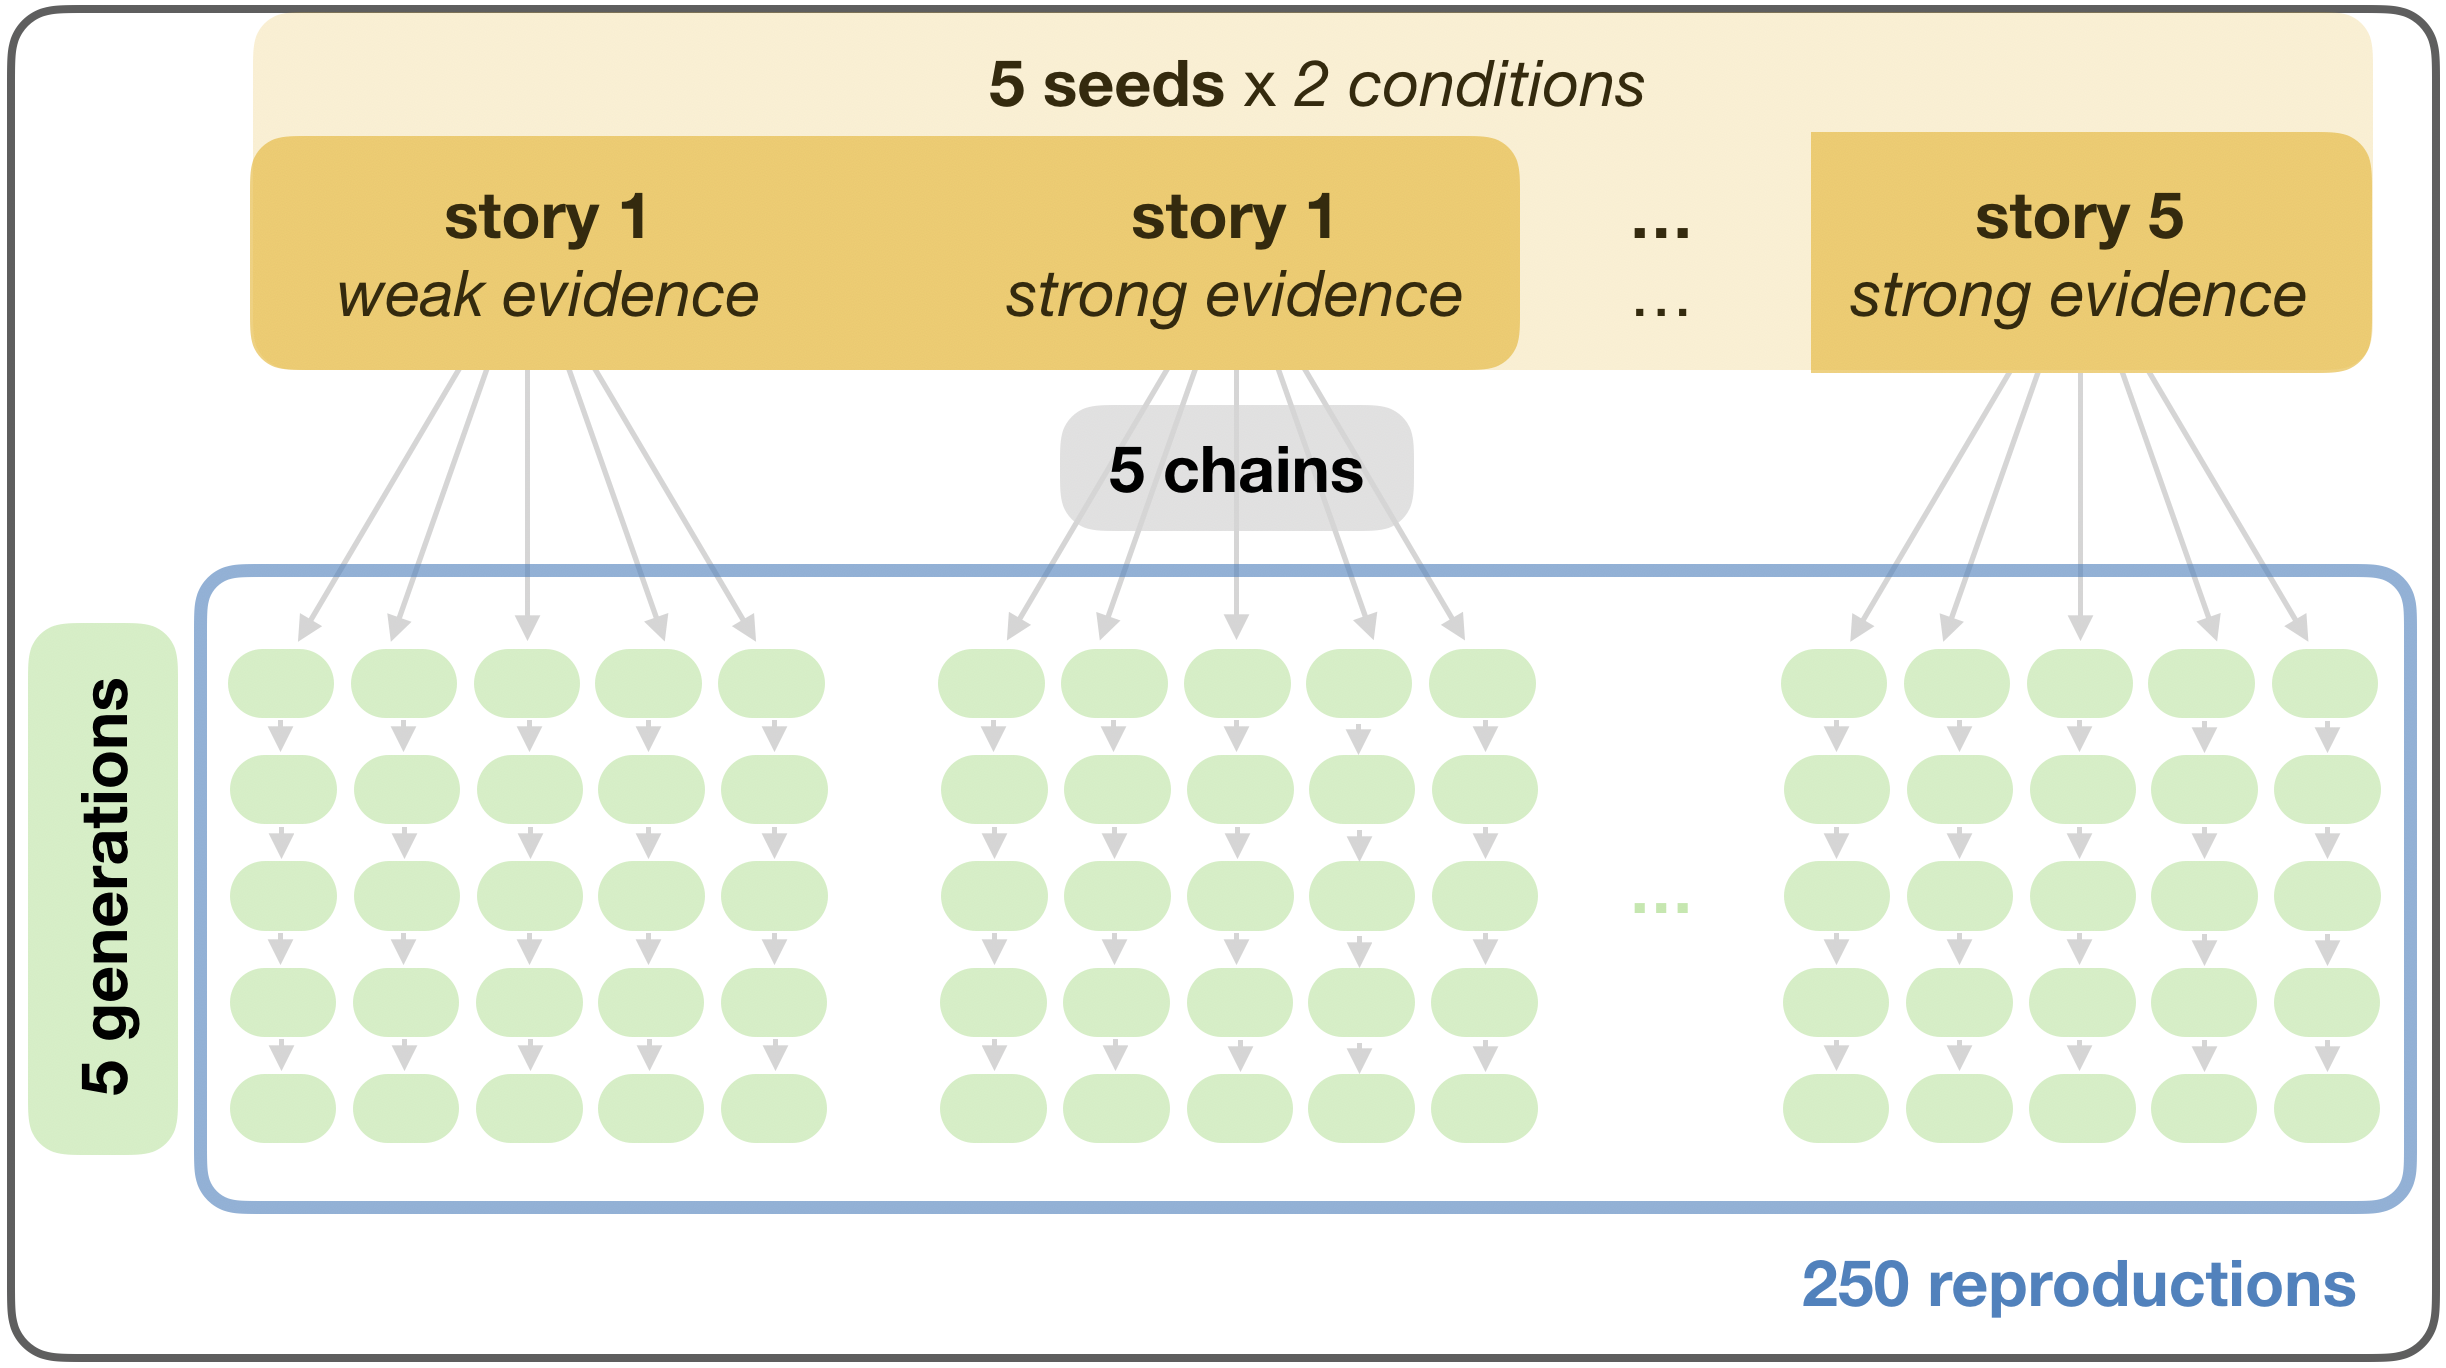
\includegraphics[width=0.48\textwidth]{pics/corpus_overview.png}
	\caption{Overview of corpus of stories collected in Exp.~1.} 
	\label{fig:design}
\end{figure}

\subsection{Results}

Participants produced 370 stories. For each seed, we defined a complete chain as one that has 5 reproductions/generations. For subsequent analysis, we randomly selected 50 complete chains, evenly distributed across stories and conditions. This yielded a corpus of 250 reproductions (5 seeds in 2 conditions with 5 complete chains each, see Figure \ref{fig:design}). This was the maximal set of complete chains that was present in every condition for each seed. This corpus is a rich source of linguistic information which merits detailed investigation. Yet, with an eye to clear operationalizability, we focus here on a few general features, which we will subsequently use as predictors in the analyses of Exp.~2 below.

\textbf{Proportion of hedges.} As a proxy for vagueness, we extracted the number of hedges per story relative to its length. The seed stories were designed to contain various hedges, such as "nearly", "about", "up to" or "allegedly". As shown in Figure \ref{fig:corpusLingMetrics}, the proportion of hedges decreased in each generation  ($\beta = -0.01$, $SE = 0.00$, $t = -4.16$, $p < 0.0001$), suggesting that participants portrayed the stories with more certain language over generations. There was no significant effect of evidence condition on proportion of hedges.

\begin{figure*}[]
\centering
%	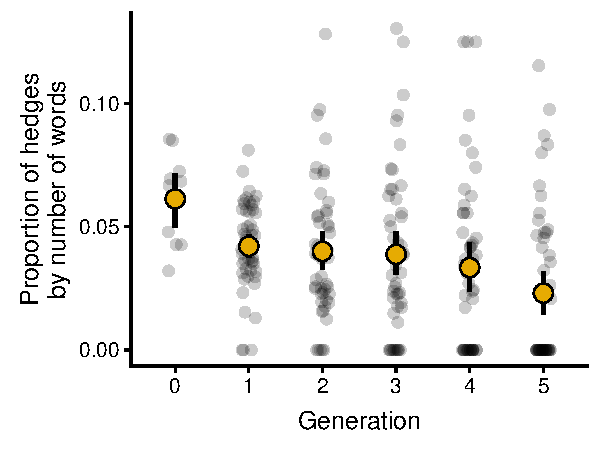
\includegraphics[width=0.48\textwidth]{pics/hedges_points.pdf}
	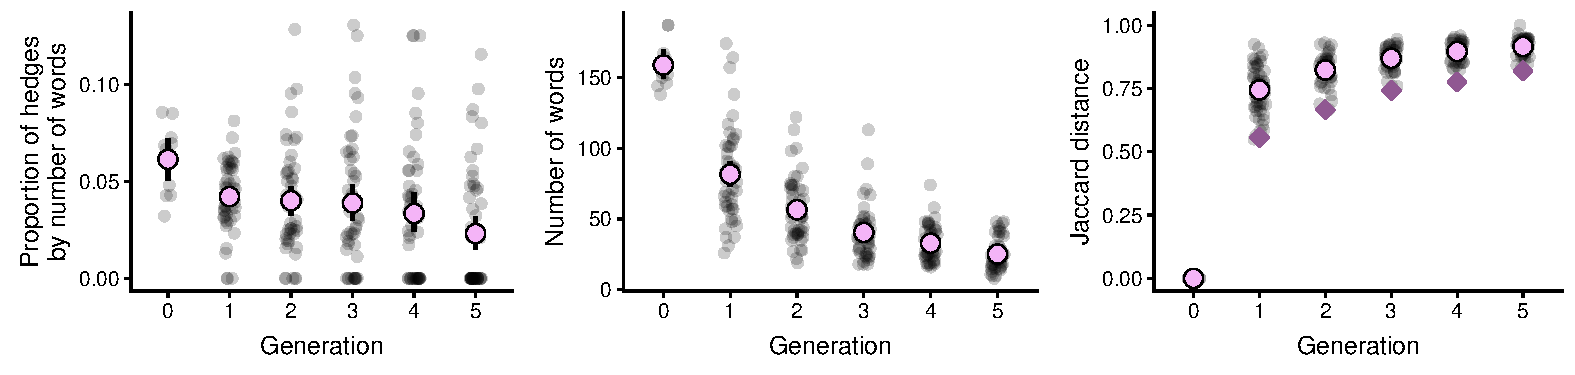
\includegraphics[width=.85\textwidth]{pics/linmeasure_grid}
	\caption{Mean of the three linguistic metrics (proportion of hedges (by number of words), number of words and Jaccard distance) over generations of reproductions. Error bars indicate bootstrapped 95\% CIs. Orange dots indicate generation mean, gray dots are individual stories. The red dots indicate the lowest possible distance given the mean length of the stories.} 
	\label{fig:corpusLingMetrics}
\end{figure*}

\textbf{Story length.} As shown in Figure \ref{fig:corpusLingMetrics}, the number of words in a story decreased across generations ($\beta = -17.12$, $SE = 1.02$, $t = -16.79$, $p < 0.0001$), replicating a well-known phenomenon in reproduction studies \cite{Bartlett:1932}. While the original generation 0 seeds consisted on average of 159 words, that number dropped to 25 by generation 5. Examples of reproductions of the seed in Table \ref{tab:examplestory} from generation 1 and 5 are shown in (\ref{gen1}) and (\ref{gen5}) below. There was no significant effect of evidence condition on story length.

\enumsentence{In late December 2017, a couple in Iowa went to check on their beehives.  They found a tragic scene:  their hives had been overturned and their equipment and facilities had been ransacked.  A few weeks later, the police arrested a 12-y.o. and 13-y.o. for the crime.  They are charged with multiple offenses, with fines up to \$100,000 and up to 10 years in prison, yet will be tried as minors.  The trial hasn't happened yet, but they seem guilty.\label{gen1}}
\enumsentence{A 12 and 13 year old were arrested for destroying a beehive, and face up to 10 years of jail time.\label{gen5}}

%\begin{figure}[]
%	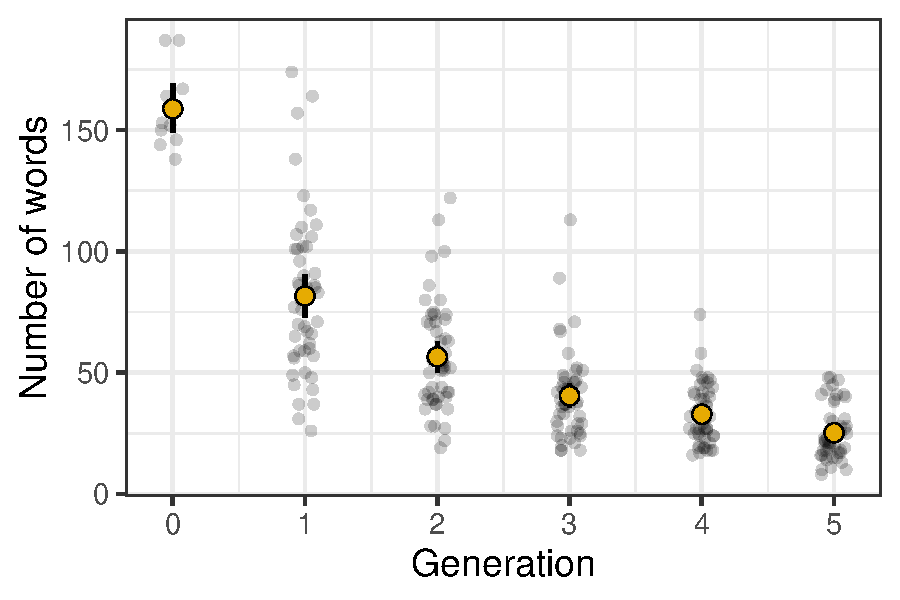
\includegraphics[width=0.48\textwidth]{pics/corpus_length.pdf}
%	\caption{Mean story length in number of words by generation in strong (left) and weak (right) evidence condition. Error bars indicate bootstrapped 95\% CIs. Orange dots indicate generation mean, gray dots are individual stories.} 
%	\label{fig:storylength}
%\end{figure}

\textbf{Similarity of seeds and reproductions.} % Of interest is the extent to which stories retain the gist or deviate from it. 
To assess the similarity between seed stories and their reproductions quantitatively, we computed the Jaccard distance between each reproduction and its generation 0 seed. Jaccard distance ranges between 0 and 1 (where 1 indicates greatest distance) and captures the amount of overlap between two stories in the following way: \[D_J(X,Y) = 1 - \frac{|X \cap Y|}{|X \cup Y|}\] where X is the set of words in the reproduction and Y the set of words in the respective original seed story. In this case, we took words as the basic unit over which distance was computed. Figure \ref{fig:corpusLingMetrics} shows that $D_J$ increased across generations ($\beta = 0.05$, $SE = 0.00$, $t = 14.17$, $p < 0.0001$). This is not surprising given that as story length decreases, $D_J$ between seed and any of its reproductions necessarily increases. However, we will see later that length and $D_J$ have different effects on story interpretation. There was no significant effect of evidence condition on Jaccard distance. %However, $D_J$ increased more strongly than expected if the difference between stories was only due to the decrease in length \ek{is this true?} \mf{this is tricky. I wouldn't know how to \emph{quickly} check this; first thing that comes to mind is, unsurprisingly, simulation; we could sample random subsets of words corresponding to the mean story lengths and check JD for that; but that's time consuming and I don't think that this is worthwhile currently; I'd rather suggest we formulate this differently, weaker, less prone to criticism if we do not back it up}, suggesting that information was lost across generations. This can also be observed qualitatively in the comparison of the representative examples (\ref{gen1}) and (\ref{gen5}) above.

%\begin{figure}[]
%	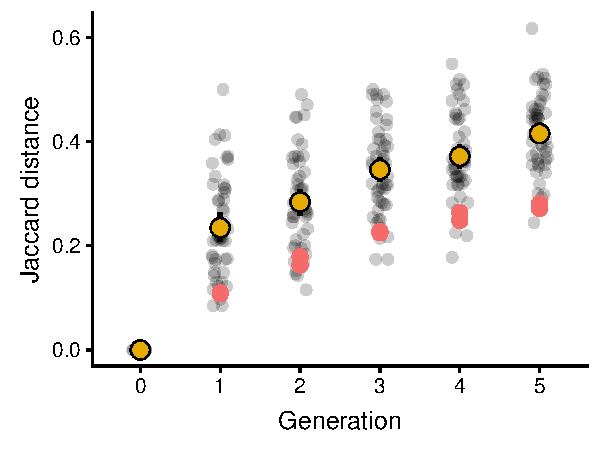
\includegraphics[width=0.48\textwidth]{pics/jaccdistance.pdf}
%	\caption{Mean Jaccard distance between seed and reproductions by generation in strong (left) and weak (right) evidence condition. Error bars indicate bootstrapped 95\% CIs. Orange dots indicate generation mean, gray dots are individual stories, red dots indicate the lowest possible distance given the mean length of the stories.} 
%	\label{fig:jaccdistance}
%\end{figure}

In sum, in a corpus of 250 reproductions of 5 seed stories, the length of the stories, the similarity to the seed story, and the proportion of hedges decreases over generations, regardless of the initial evidence strength condition.

\section{Experiment 2: story ratings}

In order to assess the extent to which, as a function of the originally provided evidence, the generation of reproduction affects readers' interpretation of various features of the stories we collected judgments from a second group of independent participants. We were particularly interested in features related to the uncertainty of presented evidence and the associated judgments of suspect guilt. We also collected judgments concerning the readers' general attitude towards the author and the story.

\subsection{Methods}

5392 participants were recruited over Amazon Mechanical Turk. Each participant read one story from the 250 story corpus reported in the previous section, and answered twelve questions about the story (including four attention checks). They indicated their response by moving a slider on a continuous scale (slider endpoints were underlyingly coded as 0 - 100). Each question was shown in isolation in a randomized order. Participants spent on average two to three minutes on this experiment and were paid \$0.60 (\$12-\$18 per hour). The story was visible throughout the experiment.


The list of questions asked is provided in (\ref{q1}) to (\ref{q8}). Questions (\ref{q1}) - (\ref{q5}) assessed the extent to which the reader believes the suspect(s) is/are guilty of the alleged crime. Questions (\ref{q6}) - (\ref{q8}) assessed the  reader's trust in the author, the extent to which they considered the story to be objectively written, and the extent to which they felt emotionally connected to the story. Overall, participants were asked eight questions of interest and four attention check questions designed to filter out participants who were just clicking through the experiment. %The attention checks were counterbalanced and asked about the likelihood that the passage is a Greek fairy tale, a Bible quote, contains more than five words, and that the story involves \textit{X}, where X was replaced by a topic which was likely to occur in the story (e.g., \textit{bees} for the story in Table \ref{tab:examplestory})

\enumsentence{How strong is the evidence for the suspect's / suspects' guilt?\label{q1}}
\vspace{-.5cm}
\enumsentence{How likely is it that the suspect is / the suspects in the crime are guilty?\label{q2}}
\vspace{-.5cm}
\enumsentence{How likely is a conviction of the suspect(s) in the crime?\label{q3}}
\vspace{-.5cm}
\enumsentence{How justified would a conviction of the suspect(s) in the crime be?\label{q4}}
\vspace{-.5cm}
\enumsentence{How much does the author believe that the suspect is guilty?\label{q5}}
\vspace{-.5cm}
\enumsentence{How much do you trust the author?\label{q6}}
\vspace{-.5cm}
\enumsentence{How objectively / subjectively written is the story?\label{q7}}
\vspace{-.5cm}
\enumsentence{How affected do you feel by the story?\label{q8}}


\subsection{Results}

\textbf{Exclusions.} We excluded 12 participants because they completed the study multiple times and another 535 because they failed at least two of the attention check questions. This left us with 4573 participants (84.8\% of the original set). After exclusions, each reproduction received on average 17 ratings, ranging from 9 to 22 and two outliers with 27 and 38 ratings. %\footnote{The outliers are due to a mistake in the recruitment process.}. 
The original seed stories received between 25 and 31 ratings.

%\jd{remind people of main question and how it will be addressed}

\textbf{Analysis procedure.} Of main interest was whether participants give judgments of suspect guilt in line with the originally provided evidence, whether those judgments change over generations, and whether those judgments pattern with related measures of evidence for guilt, probability of conviction, justification of conviction, and attributed suspect guilt (i.e., an estimate of the author's belief in the suspect's guilt). We refer to these measures as \emph{guilt related measures}. Additionally, we analyzed trust in the author, story subjectivity, and emotional engagement as measures of secondary interest. Mean slider ratings corresponding to the analyses are shown in Figure \ref{fig:exp2results}.  Judgments were analyzed using linear mixed effects models. For each question, slider rating was predicted from fixed effects of generation, condition (reference level: strong), and their interaction. The models also included random by-story intercepts. An overview of the results is shown in Table \ref{tab:exp2results}. Each row presents the model results for one of the questions and the columns show the model outcomes for fixed effects. 


\begin{figure*}[]
	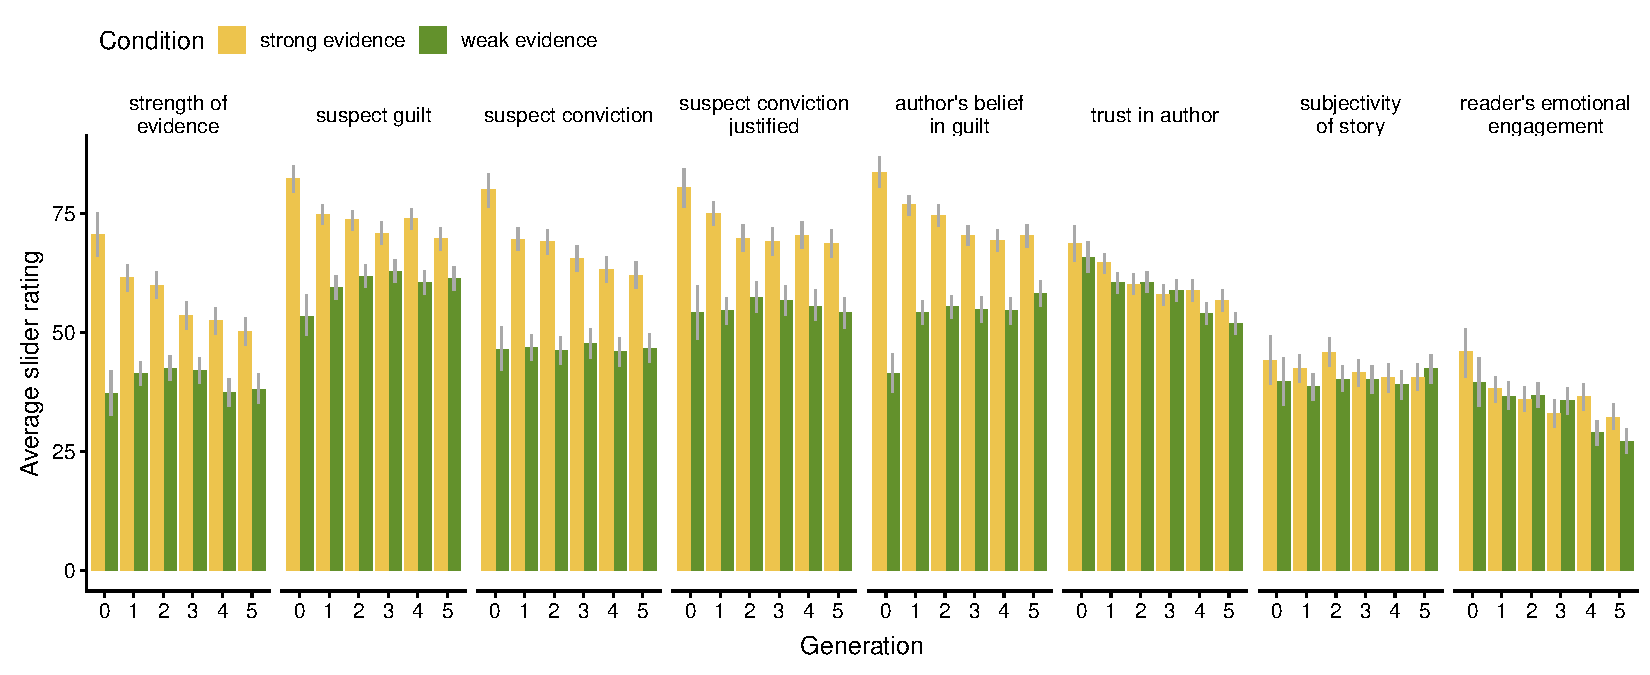
\includegraphics[width=\textwidth]{pics/subj_results_byquestion.pdf}
	\caption{Mean ratings in strong (orange) and weak (green) evidence condition for each dimension (facets).} 
	\label{fig:exp2results}
\end{figure*}

\textbf{Generation and evidence strength effects on guilt related measures.} We observed  main effects of condition on all guilt related measures (see first 5 panels of Figure \ref{fig:exp2results}), such that ratings in the strong condition were higher than ratings in the weak condition, suggesting that participants in Exp.~1 were sensitive to the evidence strength manipulation (reproducing stories in such a way that evidence strength information was maintained); and also suggesting that participants in Exp.~2 were sensitive to the reproduced evidence strength information in their judgments. %We also observed main effects or marginal main effects of generation on all 5 guilt related measures, such that ratings decreased across generation. 
We also observed significant or marginally significant interactions between condition and generation for all guilt related measures, such that ratings decreased across generations in the strong condition but remained stable in the weak condition. 


	\begin{table*}
		\centering
		\caption{Model output for each fixed effect (condition, generation, and their interaction) for each rated question (rows).}
		\vskip 0.12in
		\begin{tabular}{l r r l r r l r r l }
%		\begin{tabular}{l {p{2cm} r  p{2cm} r p{2cm} l p{2cm} r p{2cm} r p{2cm} l p{2cm} r p{2cm} r p{2cm} l }
			\toprule
			& \multicolumn{3}{c}{condition} & \multicolumn{3}{c}{generation} & \multicolumn{3}{c}{condition*generation} \\
			& \multicolumn{1}{c}{$\beta$} & \multicolumn{1}{c}{SE} & \multicolumn{1}{c}{p} & \multicolumn{1}{c}{$\beta$} & \multicolumn{1}{c}{SE} & \multicolumn{1}{c}{p} & \multicolumn{1}{c}{$\beta$} & \multicolumn{1}{c}{SE} & \multicolumn{1}{c}{p}\\
			\midrule
			strength of evidence    & -23.25 & 4.09 & $<$0.0001***        & -3.42 & 0.89 & $<$0.001*** & 2.59  & 1.26 & $<$0.05*\\
			suspect guilt          & -17.28  & 3.40 & $<$0.0001***              & -1.34 & 0.74 & $<$0.08           & 1.90  & 1.05 & $<$0.08\\
			suspect conviction   & -27.01 & 4.15  & $<$0.0001***            & -2.79 & 0.90 & $<$0.01**     & 2.74  & 1.28 & $<$0.05*\\
			suspect conviction justified    & -19.02 & 4.35 & $<$0.0001***  & -1.69 & 0.95 & $<$0.08      & 1.43 & 1.34 & $<$0.29\\
			author's belief in guilt     & -27.53 & 3.72 & $<$0.0001***     & -2.14 & 0.81 & $<$0.01**      & 3.42  & 1.15 & $<$0.01**\\
			trust in author           & -0.82   & 2.25 & $<$0.72                  & -1.94 & 0.49 & $<$0.001*** & -0.54 & 0.70 & $<$0.44 \\
			subjectivity of story  & -6.12   & 2.21 & $<$0.01**                 & -0.86 & 0.49 & $<$0.08         & 1.40   & 0.69 & $<$0.05*\\
			reader's emotional engagement  & 0.85   & 2.99 & $<$0.78   & -1.49 & 0.65 & $<$0.05*     & -1.11  & 0.92 & $<$0.24\\
					\bottomrule
		\end{tabular}
		%\caption{lmer(suspectconvictionJustified ~ generation * condition + (1|storyreproduction), data=dfmodel); high correlation of fixed effects}
		\label{tab:exp2results}
	\end{table*}



\textbf{Generation and evidence strength effects on secondary measures.} The secondary measures look very different from the guilt related measures. In particular, there were no significant effects of evidence strength condition on any of the measures with the following exception: stories were rated as less subjective in the weak evidence condition in earlier generations, though subjectivity ratings did not vary as a function of generation and remained on the `objective' side of the scale throughout. In contrast, both trust in the author and readers' emotional engagement with the story decreased across generations. This is presumably the result of the stories becoming shorter over generations (see Exp.~1) and readers therefore having less material to be emotionally affected by, and less material to build trust in the author on in later generation stories.

\textbf{Preliminary discussion.} If one expected trust in the author, the subjective quality of the story, or the reader's emotional engagement with the story to be an important factor in readers' assessment of the described suspects' guilt, one would be disappointed. The guilt related measures are entirely uncorrelated with the secondary measures. The evidence strength effect was expected, given the strong manipulation in the final sentence of the seed story. However, what is it that changes over generations that affects the guilt related measures in the strong and weak evidence conditions differently? What changes is the content of the stories. We next report a second set of analyses  in which we assess the extent to which the linguistic features reported in Exp.~1 predict ratings in Exp.~2, focusing on the readers' assessment of suspect guilt and of attributed suspect guilt.

\textbf{Effects of linguistic features on suspect guilt and author belief in suspect guilt.} 
 In this part of the analysis, we focus on the measures of \textit{suspect guilt} and \textit{author's belief in guilt} (attributed suspect guilt). These measures are interesting to examine in more detail because a) suspect guilt is the main issue raised in the 5 seed stories, so it is relevant to understand the linguistic conditions that lead to changes in perceived guilt; and b) while there is no obvious reason why readers' ultimate beliefs and the beliefs they ascribe to the author \emph{should} differ after reading these stories, \shortciteA{Degen2019} showed that listeners maintain uncertainty about the state of the world even when they ascribe a strong belief to speakers. In the following, we therefore analyze for both measures the effect of the proportion of hedges in a story, story length, and dissimilarity between a story and its seed.

Results are shown in Figure \ref{fig:lingmarkers}. In order to analyze the effects of proportion of hedges, story length, and Jaccard distance on the two guilt measures of interest, we asked whether the linguistic features explained variance above and beyond generation. To assess this, we first residualized each feature against generation, due to the substantial correlations between the features and generation observed in Exp.~1. The final mixed effects linear regression models predicted slider rating for each of the two measures and each of the three linguistic features of interest from main effects of evidence strength condition, residualized linguistic feature, generation, the interaction between evidence strength condition and generation, and the interaction between evidence strength condition and residualized linguistic feature. \footnote{Nested model comparison revealed that the inclusion of the residualized linguistic feature fixed effects were justified in all cases.}

\begin{figure}[]
	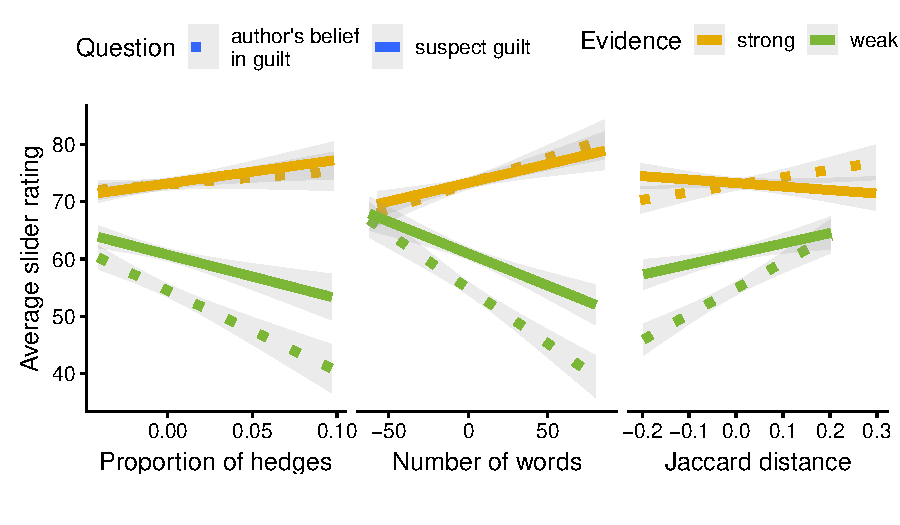
\includegraphics[width=.5\textwidth]{pics/lingmarkers_resid}
	\caption{Linearly smoothed mean slider ratings as a function of generation-residualized proportion of hedges in story (left), number of words (middle), and Jaccard distance (right). Suspect guilt ratings shown in solid lines, author belief in suspect guilt ratings shown in dashed lines. Gray ribbons indicate 95\% confidence intervals.} 
	\label{fig:lingmarkers}
\end{figure}

We observed significant interactions between evidence strength condition and generation-residualized linguistic feature for all three linguistic features for both attributed suspect guilt (hedge proportion: $\beta = -162.93$, $SE = 58.98$, $t = -2.76$, $p < .01$, story length: $\beta = -0.30$, $SE = .06$, $t = -4.38$, $p < .0001$, Jaccard distance: $\beta = $, $SE = $, $t = $, $p < $) and suspect guilt (hedge proportion: $\beta = -111.54$, $SE = 54.5$, $t = -2.05$, $p < .05$, story length: $\beta = -0.18$, $SE = .06$, $t = -2.93$, $p < .01$, Jaccard distance: $\beta = $, $SE = $, $t = $, $p < $). 


The model comparison revealed that a model which includes any of the linguistic metrics predicts \textit{author's belief in guilt} significantly better than the baseline \ek{include stats}. This holds similarly for \textit{suspect guilt} when including the Jaccard distance and length, but not the proportion of hedges \ek{include stats}. Figure (\ref{fig:lingmarkers}) visualizes the differences between questions and conditions for each of the linguistic metrics. Simple effects analysis revealed that none of the linguistic metrics has an effect in the strong condition. However, in the weak evidence condition an increase in proportion of hedges and number of words significantly decreases the guilt rating overall. In the same condition, increasing Jaccard distance results in higher guilt ratings.\\
Even though the question about \textit{suspect guilt} and \textit{author's belief in guilt} receive very similar ratings in the strong conditions, the weak condition shows a clear distinction. Overall participants judge the suspect's guilt in the weak condition higher then what they consider the author's belief about the suspect's guilt. Furthermore, this difference in judgment decreases the smaller the proportion of hedges, the shorter the stories and the bigger the Jaccard distance. This suggests that the inclusion of hedges rather informs our beliefs about the author's beliefs and less about the suspect's guilt. Analogously, the bigger the Jaccard distance to the seed story, the more similar the guilt judgments become. The observations for Jaccard distance in the weak evidence condition suggest that the stories change in the direction to accommodate a reader's beliefs about the suspect's guilt. \ek{this supports the convergence to prior.}




\section{Conclusion}

\ek{insert intro sentence}

First we constructed a corpus which consists of 10 original seed stories and 250 reproductions. Half of the seed stories suggested strong and the other half weak evidence that speaks for the suspect's guilt. Our corpus collection replicates previously found effects of a decrement in length over generations of reproductions (\cite{Bartlett:1932}). Furthermore, the stories become less similar to the original seed story and the proportional number of hedges decreases.

In a second study, we obtained subjective ratings for each story regarding the question of guilt, conviction, the author of the story, the subjectivity of the story and the reader's emotional engagement. Our results suggest \textbf{\textcolor{red}{that, for one, the subtle manipulation of varying evidential strength in the original seed stories did have a lasting effect on reproductions lasting across several generations.}} We also find effects of generation. It is plausible that trust in the author and the reader's emotional engagement decrease because the reproductions become shorter with each iteration. It is less likely that this explanation holds for the generation effects in \textit{strength of evidence}, likelihood of \textit{suspect conviction} and the \textit{author's belief in the suspect's guilt}. In the ratings for these questions we see a stronger difference between conditions that the changes in length, similarity and the proportion of hedges could not account for. \ek{Therefore, it must be something about the content of the stories itself that changes.}

\textbf{\textcolor{red}{ Most interestingly, it seems that readers became, over generations, more inclined to endorse the guilt of the suspect(s) in the weak evidence condition, despite no similar increase in ratings of the strength of evidence. This may be due to a baseline or prior level of conviction that a suspect is guilty. And it would suggest that, indeed, subtle evidential information and uncertainty about evidence is washed out over several linguistic transmissions.}}

\mf{I have tried to give this some top-level interpretation, but I have to admit that I'm pretty lost when it comes to interpreting the results. }

    
%\section{Discussion}
\ek{discuss differences between stories with in- and out-group effects for smuggler and professor}
\ek{next steps?}

\mf{it is not common to have a discussion section after the conclusions. let's put it all in one section}

\bibliographystyle{apacite}

\setlength{\bibleftmargin}{.125in}
\setlength{\bibindent}{-\bibleftmargin}

\bibliography{cogsci_IN_bib}

%\begin{table*}
%	\centering
%	\begin{tabular}{l r r l r r l r r l l l l}
%		\toprule
%		& \multicolumn{3}{c}{condition} & \multicolumn{3}{c}{generation} & \multicolumn{3}{c}{condition*generation} & \multicolumn{3}{c}{simple effects}\\
%		& \multicolumn{1}{c}{$\beta$} & \multicolumn{1}{c}{SE} & \multicolumn{1}{c}{p} & \multicolumn{1}{c}{$\beta$} & \multicolumn{1}{c}{SE} & \multicolumn{1}{c}{p} & \multicolumn{1}{c}{$\beta$} & \multicolumn{1}{c}{SE} & \multicolumn{1}{c}{p} & \multicolumn{1}{c}{weak} & \multicolumn{1}{c}{str*gen} & \multicolumn{1}{c}{we*gen}\\
%		\midrule
%	    evidence    & -23.25 & 4.09 & $<$0.0001*** & -3.42 & 0.89 & $<$0.001*** & 2.59  & 1.26 & $<$0.05*  & *** & *** & \\
%		suspect guilt          & -17.28  & 3.40 & $<$0.0001*** & -1.34 & 0.74 & $<$0.08           & 1.90  & 1.05 & $<$0.08 & *** & . & \\
%		suspect conviction   & -27.01 & 4.15  & $<$0.0001*** & -2.79 & 0.90 & $<$0.01**     & 2.74  & 1.28 & $<$0.05*  & *** & ** & \\
%		conviction justified    & -19.02 & 4.35 & $<$0.0001***  & -1.69 & 0.95 & $<$0.08           & 1.43 & 1.34 & $<$0.29   & *** & . &  \\
%		author's belief in guilt     & -27.53 & 3.72 & $<$0.0001***  & -2.14 & 0.81 & $<$0.01**      & 3.42  & 1.15 & $<$0.01** & *** & ** & \\
%		trust in author           & -0.82   & 2.25 & $<$0.72           & -1.94 & 0.49 & $<$0.001*** & -0.54 & 0.70 & $<$0.44   & & *** & *** \\
%		subjectivity of story  & -6.12   & 2.21 & $<$0.01**          & -0.86 & 0.49 & $<$0.08         & 1.40   & 0.69 & $<$0.05* & ** & . & \\
%		reader's emotion & 0.85   & 2.99 & $<$0.78            & -1.49 & 0.65 & $<$0.05*     & -1.11  & 0.92 & $<$0.24  & * & *** & \\
%		\bottomrule
%	\end{tabular}
%	\caption{Model output for each fixed effect (condition, generation, and their interaction) for each rated question (rows). \jd{simple effects results should not be reported in this table -- this is just here for us, right?}\ek{yes}}
%	%\caption{lmer(suspectconvictionJustified ~ generation * condition + (1|storyreproduction), data=dfmodel); high correlation of fixed effects}
%	\label{tab:exp2resultsb}
%\end{table*}

%\cleardoublepage
%\ek{TODO: condition title == facet labels}
%\begin{adjustwidth}{-1in}{-1in}

%\end{adjustwidth}

%\begin{adjustwidth}{-1in}{-1in}
%	\begin{table}
%		\centering
%		\begin{tabular}{l r r l r r l r r l}
%			\toprule
%			& \multicolumn{3}{c}{condition} & \multicolumn{3}{c}{generation} & \multicolumn{3}{c}{condition*generation}\\
%			& \multicolumn{1}{c}{$\beta$} & \multicolumn{1}{c}{SE} & \multicolumn{1}{c}{p} & \multicolumn{1}{c}{$\beta$} & \multicolumn{1}{c}{SE} & \multicolumn{1}{c}{p} & \multicolumn{1}{c}{$\beta$} & \multicolumn{1}{c}{SE} & \multicolumn{1}{c}{p}\\
%			\midrule
%			evidence                              & -23.25 & 4.09 & $<$0.0001*** & -3.42 & 0.89 & $<$0.001*** & 2.59  & 1.26 & $<$0.05*  \\
%			suspect committedCrime    & -17.28  & 3.40 & $<$0.0001*** & -1.34 & 0.74 & $<$0.08           & 1.90  & 1.05 & $<$0.08  \\
%			suspect conviction              & -27.01 & 4.15  & $<$0.0001*** & -2.79 & 0.90 & $<$0.01**     & 2.74  & 1.28 & $<$0.05*  \\
%			suspect convictionJustified & -19.02 & 4.35 & $<$0.0001***  & -1.69 & 0.95 & $<$0.08           & 1.43 & 1.34 & $<$0.29    \\
%			author belief                        & -27.53 & 3.72 & $<$0.0001***  & -2.14 & 0.81 & $<$0.01**      & 3.42  & 1.15 & $<$0.01** \\
%			author trust                          & -0.82   & 2.25 & $<$0.72           & -1.94 & 0.49 & $<$0.001*** & -0.54 & 0.70 & $<$0.44   \\
%			story subjectivity                 & -6.12   & 2.21 & $<$0.01**          & -0.86 & 0.49 & $<$0.08         & 1.40   & 0.69 & $<$0.05*  \\
%			reader emotion                    & 0.85   & 2.99 & $<$0.78            & -1.49 & 0.65 & $<$0.05*     & -1.11  & 0.92 & $<$0.24  
%			%			\bottomrule
%		\end{tabular}
%		\caption{some caption}
%		\label{tab:generationmodel}
%	\end{table}
%\end{adjustwidth}

%\begin{adjustwidth}{-1in}{-1in}
%	\begin{table}
%		\centering
%		\begin{tabular}{l r r l r r l r r l}
%			\toprule
%			& \multicolumn{3}{c}{condition} & \multicolumn{3}{c}{distance} & \multicolumn{3}{c}{condition*distance} \\
%			& \multicolumn{1}{c}{$\beta$} & \multicolumn{1}{c}{SE} & \multicolumn{1}{c}{p} & \multicolumn{1}{c}{$\beta$} & \multicolumn{1}{c}{SE} & \multicolumn{1}{c}{p} & \multicolumn{1}{c}{$\beta$} & \multicolumn{1}{c}{SE} & \multicolumn{1}{c}{p}\\
%			\midrule
%			evidence                              & -24.90 & 5.24 & $<$0.0001*** & -36.49 & 10.92 & $<$0.001*** & 27.75  & 15.41 & $<$0.08  \\
%			suspect committedCrime    & -20.12  & 4.32 & $<$0.0001*** & -14.94 & 9.00 & $<$0.10          & 26.15  & 12.71 & $<$0.05*  \\
%			suspect conviction              & -31.87 & 5.26  & $<$0.0001*** & -36.83 & 10.96 & $<$0.001***  & 39.48  & 15.47 & $<$0.05*  \\
%			suspect convictionJustified & -21.181 & 5.54 & $<$0.001***  & -21.42 & 11.55 & $<$0.07        & 19.35  & 16.30 & $<$0.24    \\
%			author belief                        & -29.90 & 4.74 & $<$0.0001***  & -9.01 & 9.87 & $<$0.37      & 39.02  & 13.94 & $<$0.01** \\
%			author trust                          & -1.19   & 2.83 & $<$0.68             & -24.73 & 5.91 & $<$0.001*** & -4.93 & 8.36 & $<$0.56   \\
%			story subjectivity                 & -6.12   & 2.77 & $<$0.05*          & -5.05 & 5.79 & $<$0.39         & 12.77   & 8.22 & $<$0.13  \\
%			reader emotion                    & 0.54   & 3.70 & $<$0.89             & -25.34 & 7.72 & $<$0.01**     & -10.44  & 10.93 & $<$0.35  
%			%			\bottomrule
%		\end{tabular}
%		\caption{lmer(suspectconvictionJustified ~ sim * condition + (1|storyreproduction), data=dfmodel); high correlation of fixed effects}
%		\label{tab:distancemodel}
%	\end{table}
%\end{adjustwidth}


%\begin{adjustwidth}{-1in}{-1in}
%	\begin{table}
%		\centering
%		\begin{tabular}{l r r l r r l r r l}
%			\toprule
%			& \multicolumn{3}{c}{condition} & \multicolumn{3}{c}{hedgesprop} & \multicolumn{3}{c}{condition*hedgesprop} \\
%			& \multicolumn{1}{c}{$\beta$} & \multicolumn{1}{c}{SE} & \multicolumn{1}{c}{p} & \multicolumn{1}{c}{$\beta$} & \multicolumn{1}{c}{SE} & \multicolumn{1}{c}{p} & \multicolumn{1}{c}{$\beta$} & \multicolumn{1}{c}{SE} & \multicolumn{1}{c}{p}\\
%			\midrule
%			evidence                              & -15.74 & 1.95 & $<$0.0001*** & 101.20 & 56.55 & $<$0.08      & -119.12  & 82.37 & $<$0.15  \\
%			suspect committedCrime    & -11.93  & 1.59 & $<$0.0001*** & 43.01 & 45.98 & $<$0.36      & -118.58  & 66.97 & $<$0.08  \\
%			suspect conviction              & -19.10 & 1.96  & $<$0.0001*** & 102.66 & 56.65 & $<$0.08  & -132.10  & 82.50 & $<$0.12  \\
%			suspect convictionJustified & -14.94 & 2.04 & $<$0.0001***  & 30.91 & 59.10 & $<$0.7        & -70.91  & 86.08 & $<$0.42    \\
%			author belief                        & -17.91 & 1.75 & $<$0.0001***  & 54.69 & 50.54 & $<$0.29      & -188.17  & 73.61 & $<$0.05* \\
%			author trust                          & -2.16   & 1.13 & $<$0.06            & 46.60 & 32.70 & $<$0.16     & 27.80 & 47.74 & $<$0.57   \\
%			story subjectivity                 & -2.22   & 1.06 & $<$0.05*          & 6.10 & 30.61 & $<$0.85         & -45.08  & 44.85 & $<$0.32  \\
%			reader emotion                    & -2.25   & 1.46 & $<$0.13             & -7.18 & 42.26 & $<$0.87     & 49.49  & 61.67 & $<$0.43  
%			%			\bottomrule
%		\end{tabular}
%		\caption{lmer(suspectconvictionJustified ~ hedgesprop * condition + (1|storyreproduction), data=dfmodel); hedges is centered; hedges = c("allegedly", "possibly", "maybe", "probably", "if", "around", "over", "nearly", "almost", "approximately", "vaguely", "up to", "roughly", "mainly", "kind of", "sort of", "kinda", "sorta", "about", "supposedly", "seem", "tend", "look like", "looks like", "appear to be", "think", "believe", "doubt", "be sure", "indicate", "suggest", "assume", "might", "perhaps", "possibility")}
%		\label{tab:hedgemodel}
%	\end{table}
%\end{adjustwidth}

%
%
%\section{General Formatting Instructions}
%
%The entire content of a paper (including figures, references, and anything else) can be no longer than six pages in the \textbf{initial submission}. In the \textbf{final submission}, the text of the paper, including an author line, must fit on six pages. Up to one additional page can be used for acknowledgements and references.
%
%The text of the paper should be formatted in two columns with an
%overall width of 7 inches (17.8 cm) and length of 9.25 inches (23.5
%cm), with 0.25 inches between the columns. Leave two line spaces
%between the last author listed and the text of the paper; the text of
%the paper (starting with the abstract) should begin no less than 2.75 inches below the top of the
%page. The left margin should be 0.75 inches and the top margin should
%be 1 inch.  \textbf{The right and bottom margins will depend on
%  whether you use U.S. letter or A4 paper, so you must be sure to
%  measure the width of the printed text.} Use 10~point Times Roman
%with 12~point vertical spacing, unless otherwise specified.
%
%The title should be in 14~point bold font, centered. The title should
%be formatted with initial caps (the first letter of content words
%capitalized and the rest lower case). In the initial submission, the
%phrase ``Anonymous CogSci submission'' should appear below the title,
%centered, in 11~point bold font.  In the final submission, each
%author's name should appear on a separate line, 11~point bold, and
%centered, with the author's email address in parentheses. Under each
%author's name list the author's affiliation and postal address in
%ordinary 10~point type.
%
%Indent the first line of each paragraph by 1/8~inch (except for the
%first paragraph of a new section). Do not add extra vertical space
%between paragraphs.
%
%
%\section{Formalities, Footnotes, and Floats}
%
%Use standard APA citation format. Citations within the text should
%include the author's last name and year. If the authors' names are
%included in the sentence, place only the year in parentheses, as in
%\citeA{NewellSimon1972a}, but otherwise place the entire reference in
%parentheses with the authors and year separated by a comma
%\cite{NewellSimon1972a}. List multiple references alphabetically and
%separate them by semicolons
%\cite{ChalnickBillman1988a,NewellSimon1972a}. Use the
%``et~al.'' construction only after listing all the authors to a
%publication in an earlier reference and for citations with four or
%more authors.
%
%
%\subsection{Footnotes}
%
%Indicate footnotes with a number\footnote{Sample of the first
%footnote.} in the text. Place the footnotes in 9~point font at the
%bottom of the column on which they appear. Precede the footnote block
%with a horizontal rule.\footnote{Sample of the second footnote.}
%
%
%\subsection{Tables}
%
%Number tables consecutively. Place the table number and title (in
%10~point) above the table with one line space above the caption and
%one line space below it, as in Table~\ref{sample-table}. You may float
%tables to the top or bottom of a column, and you may set wide tables across
%both columns.
%
%\begin{table}[H]
%\begin{center} 
%\caption{Sample table title.} 
%\label{sample-table} 
%\vskip 0.12in
%\begin{tabular}{ll} 
%\hline
%Error type    &  Example \\
%\hline
%Take smaller        &   63 - 44 = 21 \\
%Always borrow~~~~   &   96 - 42 = 34 \\
%0 - N = N           &   70 - 47 = 37 \\
%0 - N = 0           &   70 - 47 = 30 \\
%\hline
%\end{tabular} 
%\end{center} 
%\end{table}
%
%
%\subsection{Figures}
%
%All artwork must be very dark for purposes of reproduction and should
%not be hand drawn. Number figures sequentially, placing the figure
%number and caption, in 10~point, after the figure with one line space
%above the caption and one line space below it, as in
%Figure~\ref{sample-figure}. If necessary, leave extra white space at
%the bottom of the page to avoid splitting the figure and figure
%caption. You may float figures to the top or bottom of a column, and
%you may set wide figures across both columns.
%
%\begin{figure}[H]
%\begin{center}
%\fbox{CoGNiTiVe ScIeNcE}
%\end{center}
%\caption{This is a figure.} 
%\label{sample-figure}
%\end{figure}
%
%
%\section{Acknowledgments}
%
%In the \textbf{initial submission}, please \textbf{do not include
%  acknowledgements}, to preserve anonymity.  In the \textbf{final submission},
%place acknowledgments (including funding information) in a section \textbf{at
%the end of the paper}.
%
%
%\section{References Instructions}
%
%Follow the APA Publication Manual for citation format, both within the
%text and in the reference list, with the following exceptions: (a) do
%not cite the page numbers of any book, including chapters in edited
%volumes; (b) use the same format for unpublished references as for
%published ones. Alphabetize references by the surnames of the authors,
%with single author entries preceding multiple author entries. Order
%references by the same authors by the year of publication, with the
%earliest first.
%
%Use a first level section heading, ``{\bf References}'', as shown
%below. Use a hanging indent style, with the first line of the
%reference flush against the left margin and subsequent lines indented
%by 1/8~inch. Below are example references for a conference paper, book
%chapter, journal article, dissertation, book, technical report, and
%edited volume, respectively.
%
%\nocite{ChalnickBillman1988a}
%\nocite{Feigenbaum1963a}
%\nocite{Hill1983a}
%\nocite{OhlssonLangley1985a}
%% \nocite{Lewis1978a}
%\nocite{Matlock2001}
%\nocite{NewellSimon1972a}
%\nocite{ShragerLangley1990a}





\end{document}